\chapter{Karte \& Ökologie}
\section{Sonnensystem}
\href{http://www.weltenbau-wissen.de/sci-fi-erschaffen-fantasy-welt-erstellen-einstieg/}{Welt erstellen} \\
\href{http://www.weltenbau-wissen.de/2015/10/weltenbau-fragenkatalog-oekologie-biologie/}{Fragenkatalog} \\
\href{http://www.weltenbau-wissen.de/2015/01/weltenbau-mit-weltkarte-karte-zeichnen-tutorial/}{Weltkarte zeichnen} \\
\href{https://inkarnate.com/}{Weltenbautool}

\paragraph{Hintergedanke}
Das Ziel war es, ein System zu schaffen, welches uns erlaubt, so nahe wie möglich an den Gegebenheiten unserer Erde anzusetzen.
Dadurch wird erzielt, dass nur weniges geändert werden muss und der Großteil eins zu eins übernommen werden kann.
Besteht jedoch der Wunsch nach Änderung, so ist er immer möglich.
Im Sinne der Mystik wurde ein Planetensystem geschaffen, das ganz anders ist als unseres -- und doch ähnliche Bedingungen wie auf der Erde erlaubt.
Dazu mehr im entsprechenden Abschnitt.




\section{Planetensystem}
Wie in Abb. \ref{fig:planeten-system} zu sehen, gibt es zwei sich umkreisende Planeten, Andar und Gara, und ihren Mond Serro.
Andar und Gara drehen sich auf der gleichen Ebene um einen gemeinsamen Mittelpunkt, weshalb sie am Himmel des jeweils anderen immer an der gleichen Stelle stehen.
Dabei hat sich ihre Eigenrotation aneinander angeglichen, wodurch sie sich permanent mit der gleichen Seite ansehen (wie auch der Mond die Erde).

Damit es auch Ebbe und Flut geben kann, wird der gemeinsame Mittelpunkt von Serro auf der senkrechten Achse zur Planetenebene umkreist. 
Allerdings hält er dabei immer den gleichen Abstand zu beiden Planeten -- er hat also gleichzeitig auch die gemeinsame Bewegung auf der Planetenebene, damit dies möglich ist.

Dieses gesamte Gebilde, verdeutlicht in Abb. \ref{fig:planeten-konzept}, ist auf seiner elliptischen Sonnen-Umlaufbahn um 23 Grad gekippt, zugunsten der Existenz von Jahreszeiten.
Serro fungiert auch als Asteroidenfänger.
Somit sind die Innenseiten der Planeten schon immer verschont geblieben, allerdings ihre Außenseiten nicht.
Dort ist ab und an Gestein aus dem All eingeschlagen, weshalb die äußeren Seiten auch diverse Krater aufweisen und weniger besiedelt sind, als die Inneren.

\begin{figure}[tbh]
	\centering
	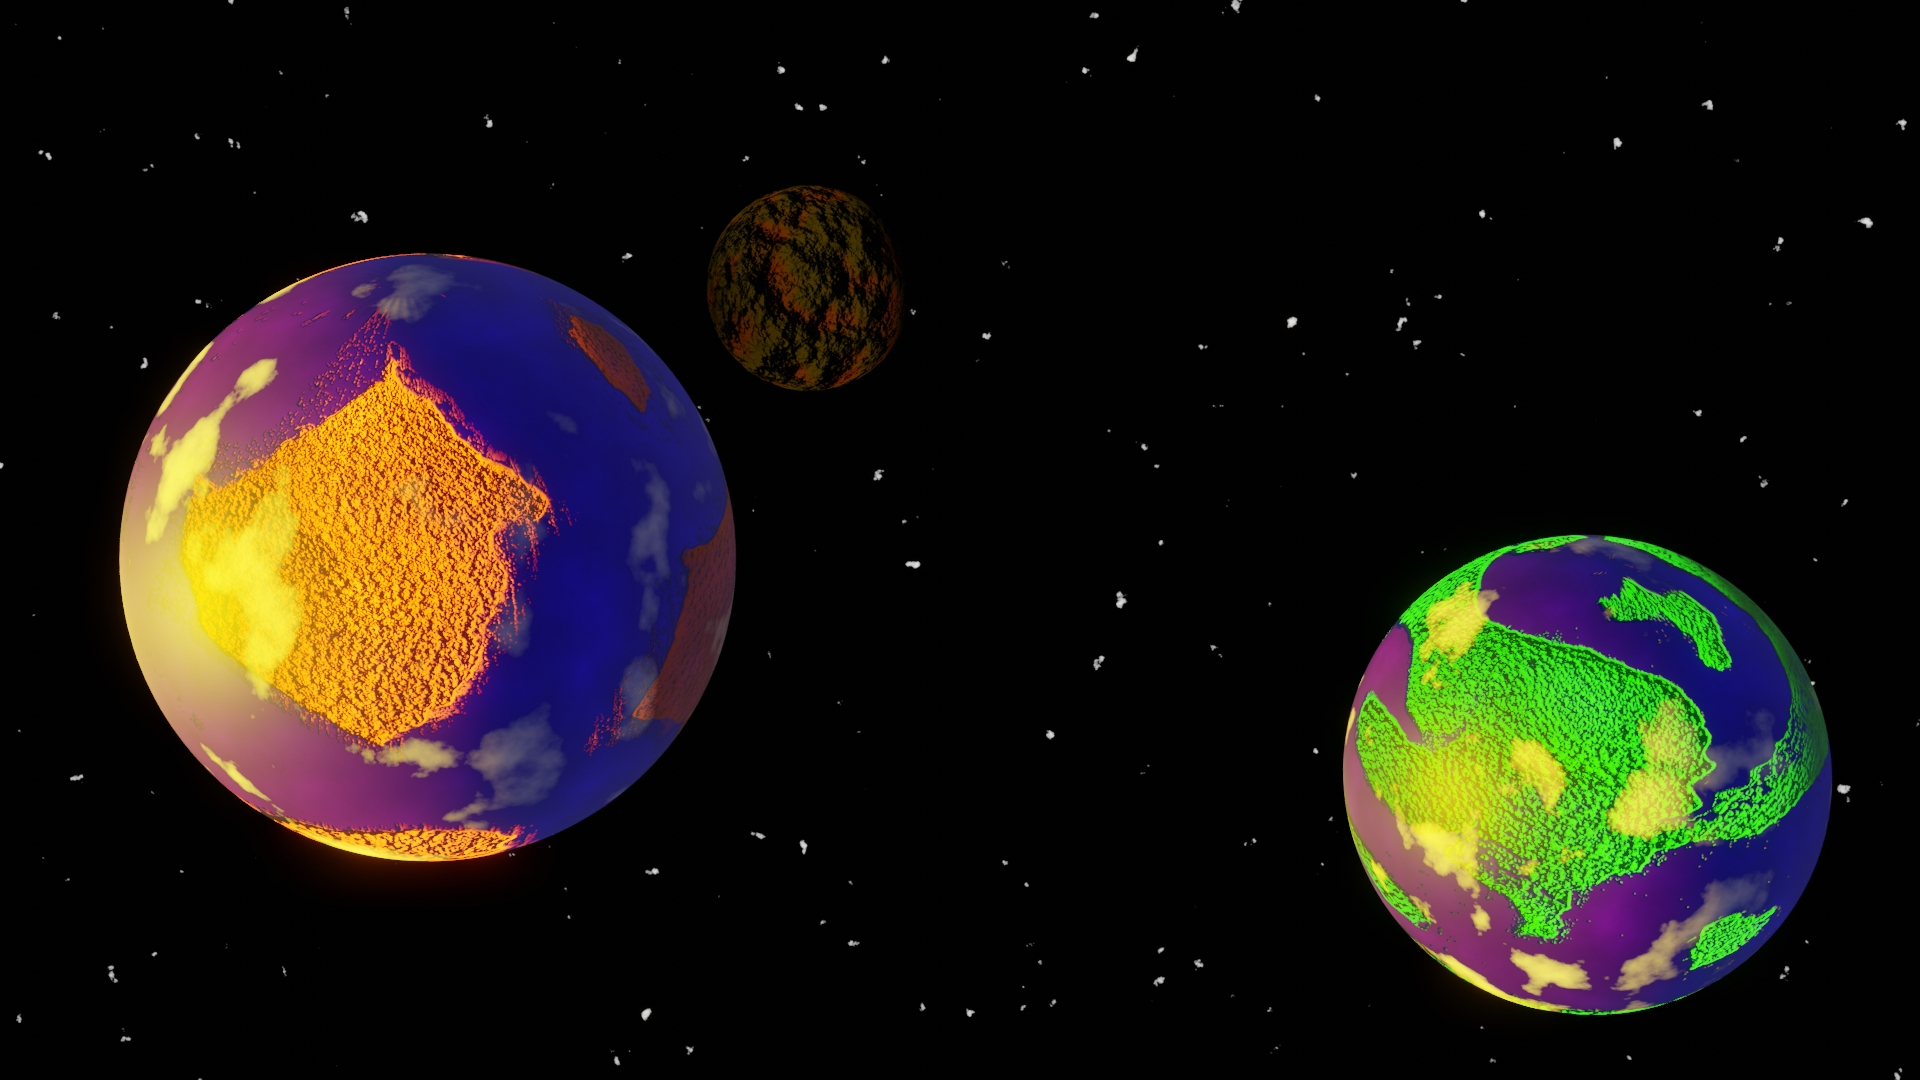
\includegraphics[width=0.9\linewidth]{Abbildungen/Weltenbau/Welt/planeten-system}
	\caption[Das Planetensystem]{\textbf{Das Planetensystem.}\\
	Die Planeten Gara (v.l.) und Andar (v.r.) mit ihrem Mond Serro (h.).}
	\label{fig:planeten-system}
\end{figure}

\begin{figure}[tbh]
	\centering
	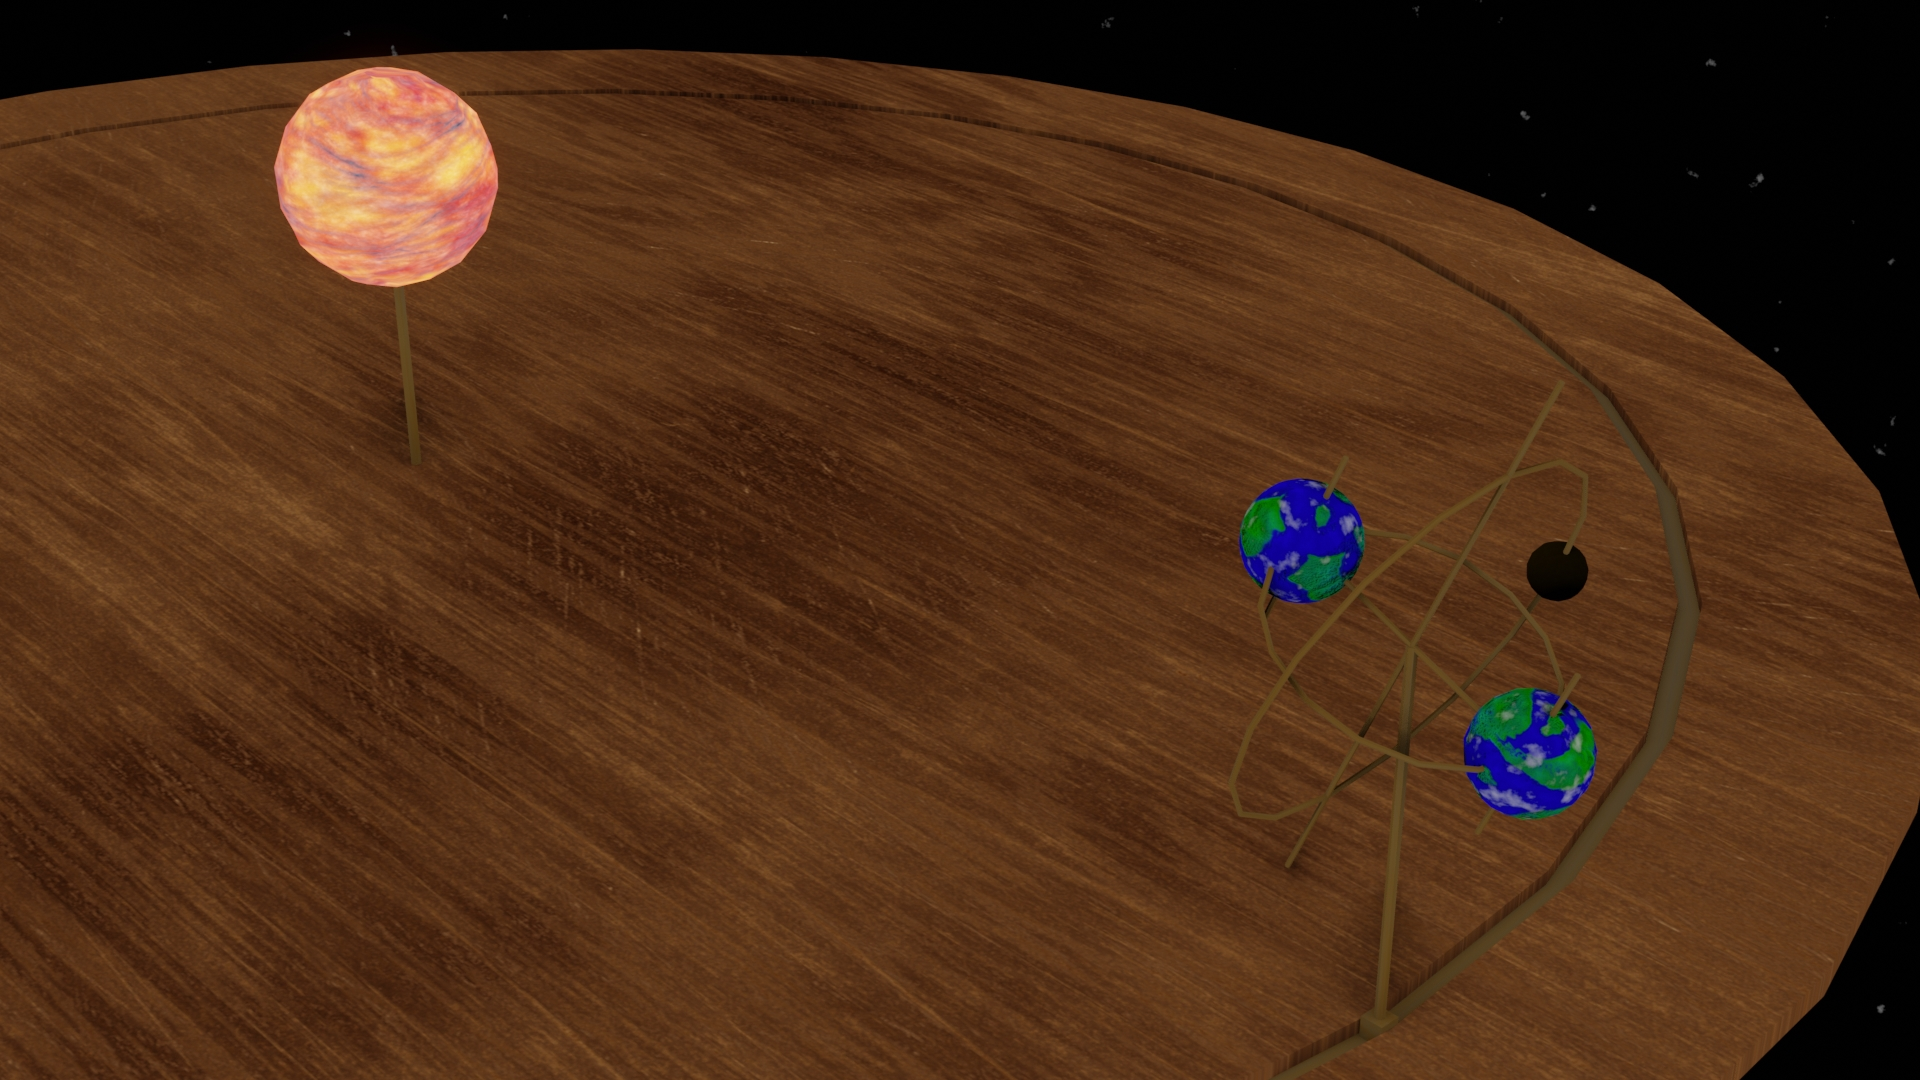
\includegraphics[width=0.9\linewidth]{Abbildungen/Weltenbau/Welt/planeten-konzept}
	\caption[Konzept des Planetensystems]{\textbf{Darstellung der Rotationsachsen des Planetensystems.}\\
	Es ist de Neigung zur Umlaufbahn um die Sonne zu sehen, als auch die Linien, auf denen sich die drei Bestandteile des Systems drehen.}
	\label{fig:planeten-konzept}
\end{figure}

\paragraph{Entstehung des Systems} 
Ähnlich zu der Entstehung von Erde und Mond sind auch Andar, Gara und Serro aus einem größeren Brocken entstanden.
Während er noch frisch und recht flüssig war, traf ihn ein anderer großer Brocken und so spalteten sie sich in drei Klumpen auf, die sich in eine stabile Rotation umeinander einfanden.
Annähernde Daten zu den Dreien finden sich in Tab. \ref{tab:planetendaten}.

\begin{table}[htb]
	\centering
	\caption[Planetendaten]{\textbf{Verschiedenste Daten zu den Planeten in der Übersicht.}}
	\label{tab:planetendaten}
	\begin{threeparttable}
		\begin{tabularx}{\textwidth}{l|ccX} %wenn die Tabelle eh schmaler als die Textbreite ist und eine rein vom Inhalt dynamische Breite gewünscht ist, muss hier und unten das x hinter tabularx sowie die zweite geschweifte Klammer entfernt werden!
			\toprule
			\textbf{1st Column} & \textbf{2nd Column} & \textbf{3rd Column} & \textbf{4th Column} \\ 
			\midrule
			Ich   &        brauche             &        noch             & die \\
			Tabelle   &       von              &          Alex           & übergeben. \\ 
			\bottomrule
		\end{tabularx}
	\end{threeparttable}
\end{table}

\paragraph{Entstehung von Leben}
Das Leben entwickelte sich auf beiden Planeten unabhängig und basiert vielleicht sogar auf völlig unterschiedlichen molekularen Grundlagen, das lassen wir an dieser Stelle offen.
Es ist einerseits vorerst nicht relevant und andererseits kann es sein, dass wir damit zukünftig noch spielen möchten.
Fest steht allerdings, dass es auf beiden Planeten zu teilweise sehr unterschiedlichen Entwicklungen kam. 


\subsection{Andar} \label{sec:planet}
Andar ist der Planet, auf dem unsere Geschichte spielt.
Seine Karte lässt sich in Abb. \ref{fig:andar-map} einsehen.
Das Leben hat sich weitestgehend so entwickelt, wie auf der Erde auch, um dem oben erklärten Prinzip zu folgen.

\begin{figure}[tbh]
	\centering
	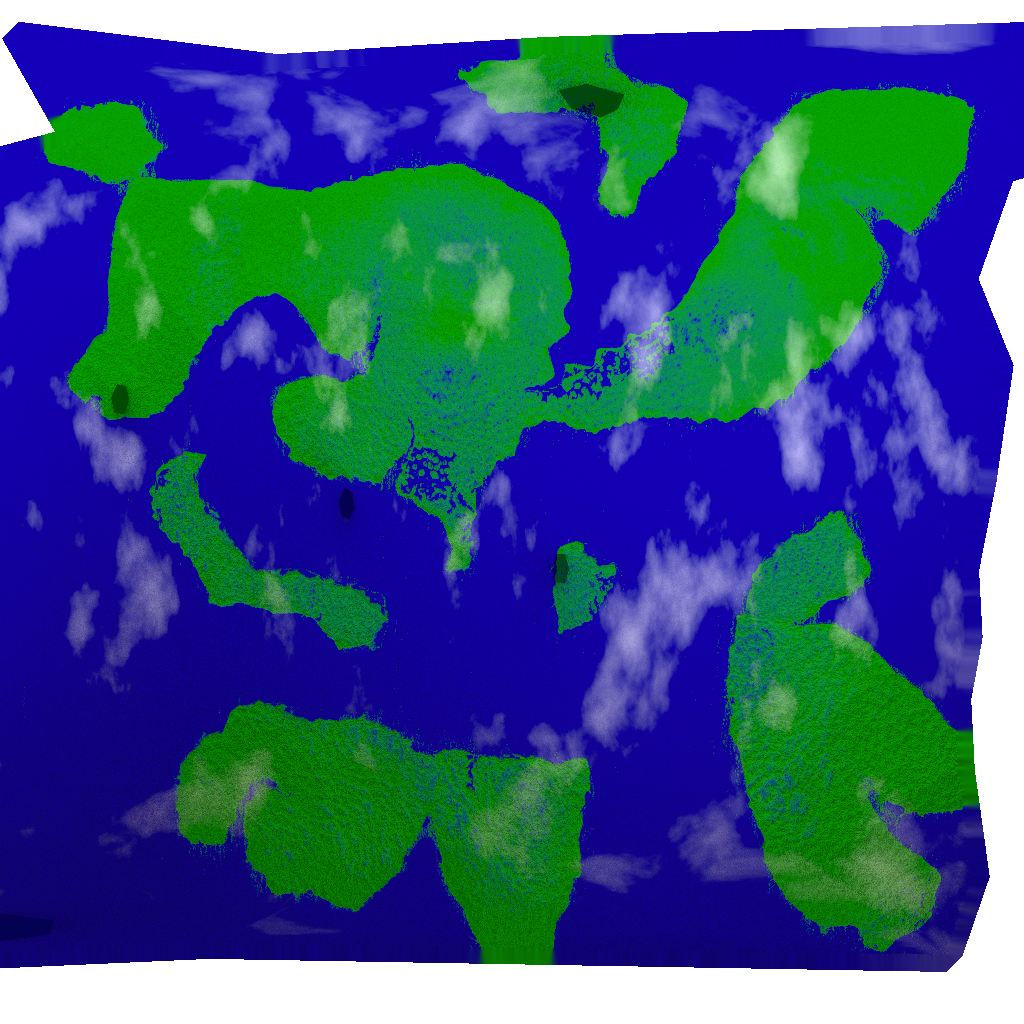
\includegraphics[width=0.7\linewidth]{Abbildungen/Weltenbau/Welt/andar-map}
	\caption[Weltkarte von Andar]{\textbf{Die Weltkarte von Andar.}}
	\label{fig:andar-map}
\end{figure}


\subsection{Gara} \label{sec:planet-zwilling}
Gara unterscheidet sich kaum von ihrem Zwilling, die größten Unterschiede liegen in der belebten Natur -- und natürlich in den Landmassen, wie Abb. \ref{fig:gara-map} zeigt.
So haben sich hier Pigmente zur Photosynthese durchgesetzt, die vor allem sämtliche Wellenlängen unter \SI{600}{\nano\meter} absorbieren.
Das demnach nicht absorbierte rot-orangene Licht bestimmt auf Gara die Farbgebung der Flora.
Weiterhin hat sich nach der Eroberung des Landes eine weitere Pigmentfamilie durchgesetzt, welche Wellenlängen über \SI{500}{\nano\meter} absorbiert und so für eine lila-blaue Erscheinung sorgt.

\begin{figure}[tbh]
	\centering
	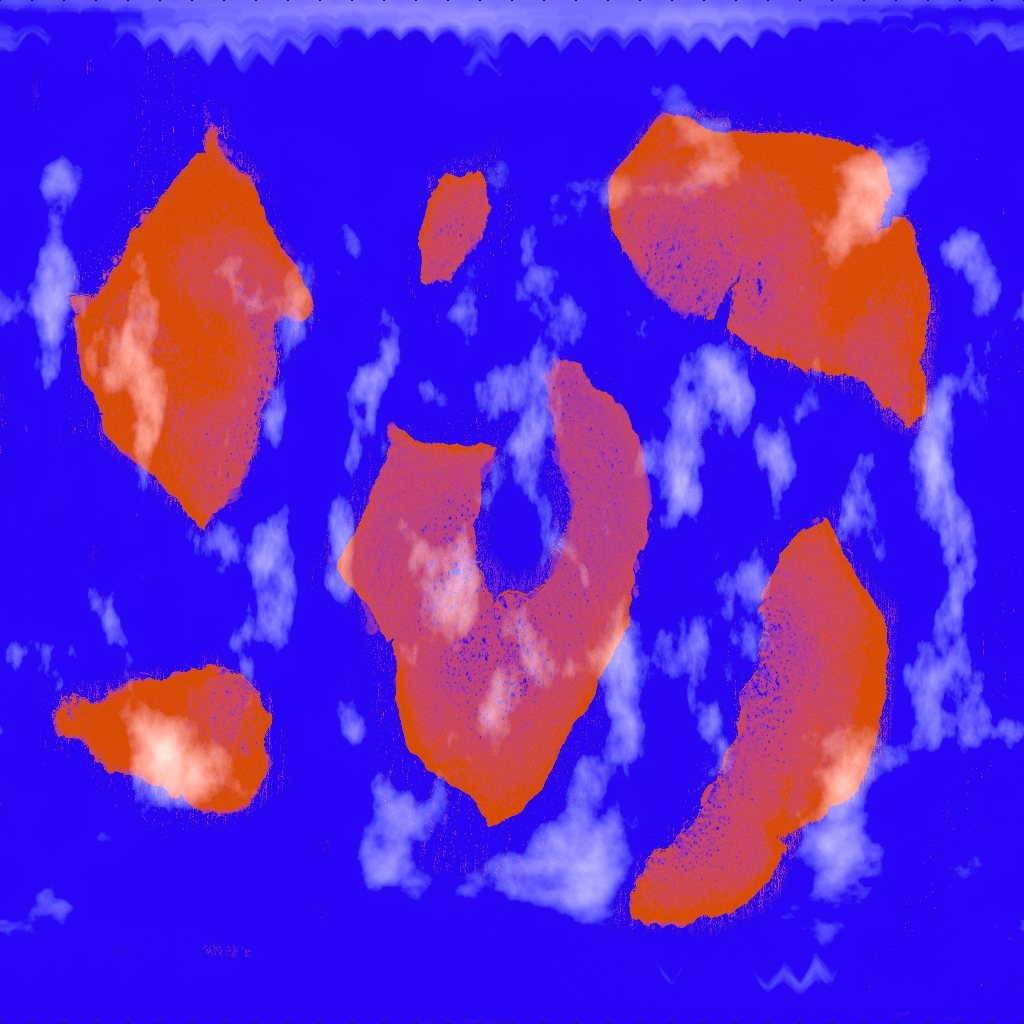
\includegraphics[width=0.7\linewidth]{Abbildungen/Weltenbau/Welt/gara-map}
	\caption[Weltkarte von Gara]{\textbf{Die Weltkarte von Gara.}}
	\label{fig:gara-map}
\end{figure}


\subsection{Serro} \label{sec:mond}
Serro ist ein Gesteinsbrocken, dessen Zusammensetzung aus Gestein und metallischen Erzen für sein charakteristisches Erscheinungsbild sorgt.



\section{Kontinent}
Der Kontinent auf dem wir sind ist Teil von der Landmasse, die sich einmal um den ganzen Planeten spannt.
Er befindet sich auf mittleren Breitengraden ziemlich mittig bezüglich des Mittelpunktes des Planetensystems.
Dadurch haben wir dort etwa mitteleuropäische Voraussetzungen was Jahreszeiten und Temperaturen anbelangt.

\subsection{Das Riesengebirge}
Ein gigantisches Gebirge, das Riesengebirge, prägt das Bild des Kontinents.

\subsection{Gigantus Wald} \label{sec:gigantuswald}
\begin{outline}
	\1 wie bekannt, können auch Pflanzen die ihnen innewohnende Magie nutzen. Eine Art (!!) von Bäumen haben folgendes entwickelt: sie ermöglichen mittels der Magie die Wasserversorgung der oberen Baumabschnitte gegen die Gravitation. Das Größeneinschränkende Element normaler Bäume ist damit weg. Daher konnten die Bäume extrem groß werden, bevor weitere Prozesse ihr Wachstum stoppten und hatten damit den Platz an der Sonne sicher
	\1  diese Garganten (Working title) erreichen Höhen von 500m und ähnlich wie aus dem Dschungel bekannt, bilden sich somit verschiedene vertikale Lebensbereiche
	\1 der Boden ist bedeckt mit allerlei Gehölz und Sträuchern, die wenig Sonnenlicht brauchen, und ganz vorne voran riesigen Pilzen, die in Symbiose mit den riesigen Bäumen ebenfalls ein gigantisches unterirdisches Netzwerk bildeten und nun gigantische Fruchtkörper (:mushroom:  das da) ausbilden können
	\1 die ersten kräftigen Äste der Garganten haben stark grüne, mit viel Chlorophyll gefüllte Blätter, die jegliches Licht, das durch die oberen Schichten kommt, aufnehmen kann. Für unsere Verhältnisse stehen die Bäume zwar ewig weit auseinander, doch auf ein normales Größenverhältnis reduziert nicht. Ihre Äste können sich an den Spitzen erreichen und bilden so mittels der Äste und den riesigen Laubblättern eine Art zweiten Boden, beginnend in 200m Höhe
	\1 durch die Ausmaße der Äste sammelt sich Erde hier und dort und es wachsen normale Bäume auf dieser Ebene, allerdings nicht zu weit vom Stamm der Garganten entfernt. Ebenso finden sich hier normale Büsche etc. Schlingpflanzen ziehen sich um die dicken Äste und es bildete sich so im Laufe der Zeit in dicker "Boden" - mit unerwartete Löchern hier und da
	\1 Da wir uns hier schon in der Krone der Bäume befinden, ist ab dieser zweiten Schicht ein langsamer Verlauf in den folgenden 300m: Die Baumkrone begünstigt in ihren Ausmaßen das Wachsen anderer Bäume, Sträucher, Kräuter etc, insbesondere parasitischer Lebensformen wie Schlingpflanzen und Misteln. Auch einige "normale Bäume" wachsen nicht nur auf den Erdansammlungen, sondern auch in das Holz der Äste hinein. Insgesamt bildet sich so wie eine Art Gerüst, welches aus festen "Platformen", aus festen und wackligen Wegen horizontal, vertikal und schräg, aus Bereichen lockerer Vegetation (wie Lianen) und aus "Lichtungen" (3D, nicht 2D) besteht.
	\1 nach oben hin werden die Blätter der Garganten immer lichtdurchlässiger. Die untersten Blätter sind mehrere Meter dick und dunkelgrün vor Chlorophyll. Die obersten sind nur ein paar Zentimeter dick, kleiner, leicht hellgrün gefärbt und ansonsten Lichtdurchlässig. Das sorgt dafür, dass das Licht bis unten hin durchkommt und effizient genutzt werden kann, um den riesigen Baum (und seine Parasiten) zu versorgen
	\1 ebenso wie die Fauna, hat sich hier auch viel Getier angesammelt und angepasst in den verschiedenen Stufen. So nisten bestimmte Vögel nur in den oberen 50m der Baumkronen. Auch ein paar Menschen fanden sich hier vor langer Zeit ein und haben sich an das Leben in den Baumkronen (von 200-350m etwa) angepasst. Es ist die Heimat der \npref{rasse:sylvan}.
	\1 allerdings ist dann doch der einschränkende faktor zum einen die stabilität von holz, bevor der baum unter der eigenlast zusammenbricht, und die biegsamkeit von holz, bevor höhenwinde den baum zerbrechen. gegen letzteres könnte der baum natürlich einfach sehr dick sein. mit werten, die ich jetzt auf die schnelle für holz gefunden hab, sollte das ganze bei wenigen hundert m höhe schon instabil werden. man könnte vielleicht argumentieren, dass der baum nicht nur wasser besser transportieren kann, sondern auch mineralstoffe, um seine stabilität zu erhöhen. dann hätte man gleich ein inhärent sehr hartes holz in der welt. bei dieser höhe ist die breite auch fast egal (solange sie wenige meter überschreitet)
\end{outline}

\section{Mantodea} \label{sec:land}
\section{Tal}
\subsection{Teich 1}
\subsection{Teich 2}
\subsection{Großer Wald}
\subsection{Klippe am Eingang}

